\subsection*{Problema 01}

\textbf{Enunciado:} Probar que:
\begin{align*}
\lim_{x \to \infty} \dfrac{\ln(x)}{x} = 0 \quad \text{y} \quad \lim_{x \to 0^+} \ln(x) = -\infty
\end{align*}

\textbf{Solución:}
Para la primera parte, evaluamos el límite
\begin{align*}
\lim_{x \to \infty} \dfrac{\ln(x)}{x}
\end{align*}
el cual presenta la forma indeterminada $\frac{\infty}{\infty}$. Aplicando la regla de L'Hôpital, derivamos el numerador y el denominador respecto a $x$:
\begin{align*}
\lim_{x \to \infty} \dfrac{\frac{d}{dx}[\ln(x)]}{\frac{d}{dx}[x]} &= \lim_{x \to \infty} \dfrac{\frac{1}{x}}{1} \\
&= \lim_{x \to \infty} \dfrac{1}{x} = 0
\end{align*}
Con esto queda demostrado el primer límite.

Para la segunda parte, evaluamos el límite cuando $x$ tiende a $0^+$ del logaritmo natural:
\begin{align*}
\lim_{x \to 0^+} \ln(x)
\end{align*}
Aplicamos el cambio de variable sugerido haciendo $x = \dfrac{1}{t}$. 
Cuando $x \to 0^+$, la variable $t$ tiende a la infinidad positiva ($t \to \infty$). 
Sustituyendo en la expresión original, tenemos:
\begin{align*}
\lim_{x \to 0^+} \ln(x) &= \lim_{t \to \infty} \ln\left(\dfrac{1}{t}\right) \\
&= \lim_{t \to \infty} \left[ \ln(1) - \ln(t) \right]
\end{align*}
Sabemos que $\ln(1) = 0$, por lo que la expresión se reduce a:
\begin{align*}
\lim_{t \to \infty} \left[ 0 - \ln(t) \toBe} &= -\lim_{t \to \infty} \ln(t) \\
&= -\infty
\end{align*}
Esto completa la demostración de ambos límites solicitados.

\begin{figure}[H]
	\centering
	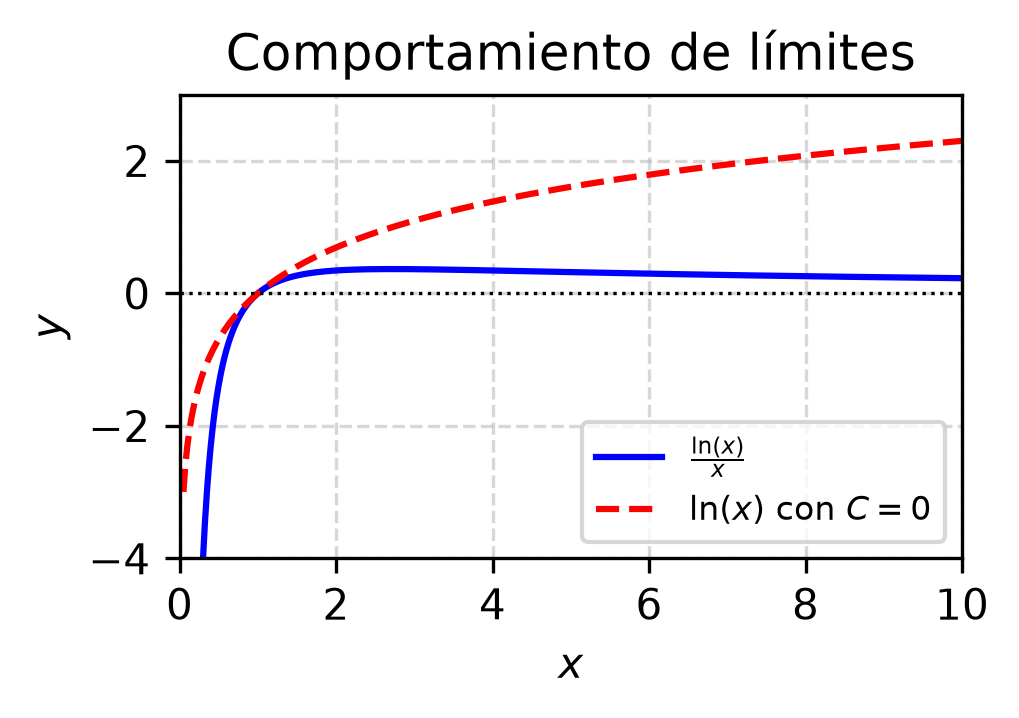
\includegraphics[width=\columnwidth]{semana_08/graficas/SEM08_P01_grafica.png}
	\caption{Representación gráfica de $f(x)$ y su antiderivada $F(x)$ evaluada para la constante de integración $C = 0$ (Problema 01).}
	\label{fig:problema01}
\end{figure}
